\documentclass[journal]{IEEEtran}

% ------------------------------------------------------------------
% Codificación e idioma
% ------------------------------------------------------------------
\usepackage[utf8]{inputenc}
\usepackage[T1]{fontenc}
\usepackage[spanish]{babel}
\usepackage{amsmath}
\usepackage{graphicx}
\usepackage{url}
\usepackage[hidelinks]{hyperref}

% Nombres en español para los elementos del formato IEEE
\renewcommand{\abstractname}{Resumen}
\renewcommand{\IEEEkeywordsname}{Términos índice}
\renewcommand{\figurename}{Figura}
\AtBeginDocument{\renewcommand{\tablename}{Tabla}}

% ------------------------------------------------------------------
% Título y autores
% ------------------------------------------------------------------
\title{Calc\_Resis\_AGBL: calculadora visual e interactiva de circuitos resistivos}

\author{
Sergio Alejandro L\'opez \'Avila\\
Andr\'es Mauricio Grajales Herrera\\
Jos\'e Esteban Monroy Santofimio\\
Cesar Alexander Su\'arez L\'opez\\
David Stevens Alfonso Villamarin
}

\begin{document}

\maketitle

% ------------------------------------------------------------------
% Resumen
% ------------------------------------------------------------------
\begin{abstract}
Este informe presenta Calc\_Resis\_AGBL, una aplicación de escritorio desarrollada por el grupo Juiciosos de UCompensar para dibujar, simular y analizar circuitos resistivos de corriente directa. La herramienta reemplaza el cálculo manual de ecuaciones por un flujo visual: el usuario agrega resistencias y fuentes de voltaje sobre un lienzo con grilla, conecta los terminales, marca la tierra y presiona el botón de resolver. A partir de la geometría del dibujo, la aplicación detecta los nodos y las ventanas del circuito, construye el sistema matricial del análisis por mallas, lo resuelve numéricamente y presenta las matrices $R$, $I$ y $V$, además de la corriente, la tensión y la potencia de cada componente. El documento explica qué hace la aplicación, cómo descargarla y ponerla en funcionamiento, el fundamento de las leyes de Kirchhoff y la evidencia de validación: 79 pruebas automatizadas, revisión estática con Ruff y un ejecutable de Windows probado. El proyecto está disponible en GitHub y se ofrece como material de apoyo para cursos introductorios de circuitos y álgebra lineal.
\end{abstract}

\begin{IEEEkeywords}
análisis por mallas, circuitos resistivos, leyes de Kirchhoff, álgebra lineal, aplicaciones de escritorio, PyQt6.
\end{IEEEkeywords}

% ------------------------------------------------------------------
% 1. Introducción
% ------------------------------------------------------------------
\section{Introducción}

El análisis de circuitos es uno de los primeros temas en los que un estudiante de ingeniería se enfrenta a la necesidad de plantear y resolver ecuaciones. En el papel, el procedimiento suele ser claro: se identifican los lazos, se aplican las leyes de Kirchhoff, se agrupan los términos y se resuelve un sistema. Sin embargo, cuando el circuito crece, el estudiante puede perder de vista la relación entre el dibujo, las ecuaciones y el resultado final. La calculadora, la regla y el lápiz permiten resolver, pero no siempre muestran \emph{por qué} el circuito se convirtió en esa matriz.

Calc\_Resis\_AGBL nace de esa dificultad. Es una aplicación de escritorio que permite dibujar un circuito resistivo de corriente directa (DC), conectarlo de forma intuitiva y obtener una solución numérica acompañada del sistema de ecuaciones que se utilizó. El objetivo no es sustituir el aprendizaje de la teoría, sino hacer visible el puente entre el circuito y el álgebra lineal: el dibujo se convierte en nodos y ramas, las ramas se organizan en mallas y las mallas producen un sistema de la forma $R \cdot I = V$.

El proyecto fue desarrollado por el grupo Juiciosos, de UCompensar, como parte de un curso introductorio de álgebra lineal. La aplicación está pensada para estudiantes que ya conocen la ley de Ohm y las leyes de Kirchhoff, pero que aún necesitan una herramienta concreta para comprobar sus cálculos y entender la estructura de la matriz. Por eso, la interfaz muestra tanto los resultados como las matrices intermedias, y permite comparar el valor obtenido por el programa con el que se obtendría a mano.

Las contribuciones principales de este trabajo son:
\begin{itemize}
  \item un lienzo interactivo para agregar, mover, rotar y conectar resistencias y fuentes de voltaje;
  \item la detección automática de nodos y de las ventanas geométricas que se usan como mallas;
  \item la construcción y resolución del sistema $R \cdot I = V$ sin que el usuario escriba ecuaciones;
  \item la presentación de las matrices, la solución y una tabla de corriente, tensión y potencia por componente;
  \item un conjunto de pruebas automatizadas y un ejecutable de Windows para facilitar su uso en clase.
\end{itemize}

El resto del informe se organiza así. La Sección~\ref{sec:que-hace} describe qué hace la aplicación y cómo se usa. La Sección~\ref{sec:descarga} explica cómo descargarla y ponerla en funcionamiento. La Sección~\ref{sec:fundamento} presenta el fundamento matemático en términos sencillos. La Sección~\ref{sec:evidencia} resume la evidencia de validación y la relación con la exposición. La Sección~\ref{sec:limitaciones} señala las limitaciones y el trabajo futuro, y la Sección~\ref{sec:conclusion} cierra el informe.

% ------------------------------------------------------------------
% 2. Qué hace la aplicación
% ------------------------------------------------------------------
\section{Qué hace la aplicación}
\label{sec:que-hace}

\subsection{Una interfaz para dibujar y resolver}

La ventana de Calc\_Resis\_AGBL se divide en cuatro zonas. A la izquierda está el panel de controles, donde se elige el tipo de componente, se escribe su valor y se selecciona el método de análisis. En el centro está el lienzo, una superficie con una grilla sobre la que se arrastran los componentes. Abajo se encuentra el panel de matrices, que muestra el sistema de ecuaciones utilizado. A la derecha aparece el panel de resultados, con la leyenda de las mallas detectadas, la tabla de corrientes, tensiones y potencias, y un resumen del componente seleccionado. La Figura~\ref{fig:ui} muestra la interfaz general.

\begin{figure*}[t]
  \centering
  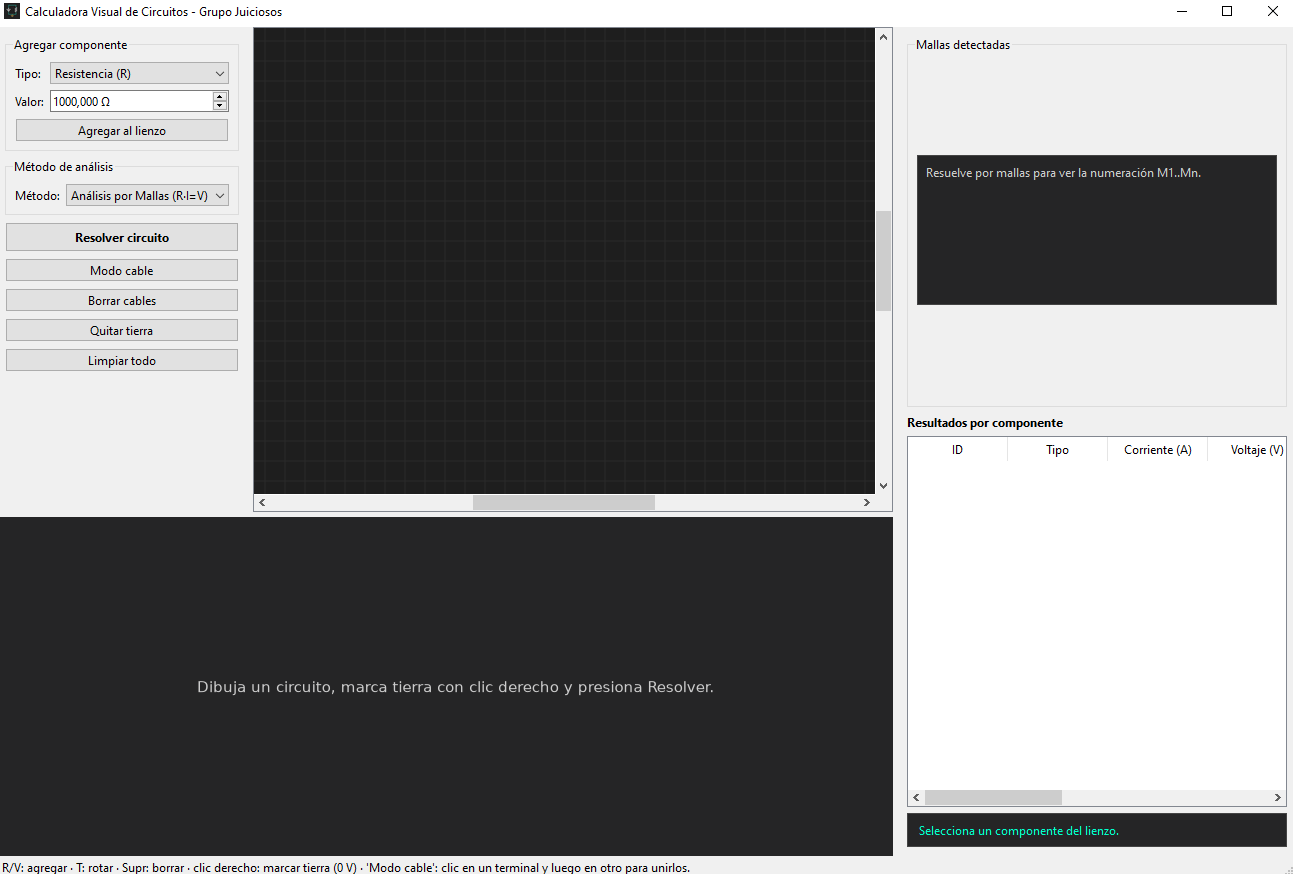
\includegraphics[width=0.86\textwidth]{../images/UI.png}
  \caption{Interfaz general de Calc\_Resis\_AGBL. Se observan el panel de controles, el lienzo central, el panel de matrices y el panel de resultados.}
  \label{fig:ui}
\end{figure*}

El flujo de trabajo es intencionalmente parecido al que se sigue en el papel. Primero se agregan los componentes: con la tecla \texttt{R} se crea una resistencia y con la tecla \texttt{E} una fuente de voltaje DC. El valor se escribe en el panel izquierdo, en ohmios para las resistencias y en voltios para las fuentes. Debajo del botón de agregar aparece un contador con el número de componentes usados, por ejemplo \texttt{Resistencias: 3/20 · Fuentes: 1/3}. Si se intenta superar un límite, la aplicación muestra un aviso y no agrega el componente; para liberar cupo basta con seleccionar uno y presionar \texttt{Supr}.

Después se ubican los componentes sobre la grilla. Cuando dos terminales quedan en la misma celda, la aplicación los interpreta como un mismo nodo eléctrico: es el llamado comportamiento de imán. Para ramas verticales, el componente seleccionado se rota 90 grados con la tecla \texttt{T}. Si los terminales están separados, se puede activar el modo cable con la tecla \texttt{W} y hacer clic en un terminal y luego en otro para tender una conexión. El modo cable es persistente y se desactiva con la misma tecla o con el botón correspondiente.

Antes de resolver, el circuito debe tener una tierra, es decir, un nodo de referencia de 0 V. La tierra se marca con clic derecho sobre un terminal o nodo y se puede quitar con el botón \emph{Quitar tierra}. Este paso es importante porque sin una referencia el problema no está bien definido. Si falta la tierra, si hay nodos desconectados o si el circuito no tiene ninguna malla cerrada, la aplicación muestra un mensaje de error en lugar de inventar un resultado.

\subsection{Qué se obtiene al resolver}

Al presionar \emph{Resolver circuito} con el método de mallas, la aplicación construye el sistema y lo resuelve. En el panel inferior se muestran tres matrices apiladas: $R=$, $I=$ y $V=$, con las filas y columnas rotuladas $M_1, M_2, \ldots$ para identificar cada malla. Debajo aparece la línea de solución con el valor numérico de cada corriente de malla. En el panel derecho, la leyenda \emph{Mallas detectadas} indica qué componentes pertenecen a cada ventana y en qué sentido se recorrió. Finalmente, la tabla de resultados lista cada elemento con su identificador, tipo, corriente, voltaje y potencia.

La Tabla~\ref{tab:atajos} resume los atajos principales y la Tabla~\ref{tab:limites} recuerda los límites de la versión actual. Estos límites son deliberados: mantienen la interfaz manejable y permiten que el proyecto se centre en los conceptos de mallas y álgebra lineal, sin convertirse en un simulador profesional de circuitos.

\begin{table}[t]
  \caption{Atajos de teclado principales.}
  \label{tab:atajos}
  \centering
  \small
  \begin{tabular}{@{}ll@{}}
    \hline
    Tecla & Acción \\
    \hline
    \texttt{R} & Agregar una resistencia \\
    \texttt{E} & Agregar una fuente DC \\
    \texttt{T} & Rotar 90° el componente seleccionado \\
    \texttt{W} & Activar o desactivar el modo cable \\
    \texttt{Supr} & Borrar el componente seleccionado \\
    Clic derecho & Marcar tierra (0 V) \\
    \hline
  \end{tabular}
\end{table}

\begin{table}[t]
  \caption{Límites de la versión actual.}
  \label{tab:limites}
  \centering
  \small
  \begin{tabular}{@{}lcc@{}}
    \hline
    Componente & Máximo & Al superar el tope \\
    \hline
    Resistencias & 20 & Aviso y bloqueo \\
    Fuentes DC & 3 & Aviso y bloqueo \\
    \hline
  \end{tabular}
\end{table}

% ------------------------------------------------------------------
% 3. Descarga y puesta en marcha
% ------------------------------------------------------------------
\clearpage
\section{Cómo descargarla y ponerla en marcha}
\label{sec:descarga}

El proyecto está publicado en el repositorio de GitHub:
\begin{center}
  \url{https://github.com/SergLopz/Calc_Resis_AGBL}
\end{center}

Existen dos formas de usar la aplicación. La primera está pensada para quien solo quiere abrirla en Windows y no quiere instalar herramientas de desarrollo. La segunda está pensada para quien quiere ejecutarla desde el código fuente, revisar el proyecto o generar su propio ejecutable.

\subsection{Opción A: paquete para Windows}

El equipo generó un paquete comprimido para Windows de 64 bits. Si se recibe el archivo \texttt{CalcResisAGBL-windows-x64.zip}, el procedimiento es el siguiente:
\begin{enumerate}
  \item descomprimir el ZIP en una carpeta local;
  \item conservar juntos el archivo \texttt{CalcResisAGBL.exe} y la carpeta \texttt{\_internal};
  \item ejecutar \texttt{CalcResisAGBL.exe}.
\end{enumerate}

No es necesario instalar Python ni las librerías del proyecto: el paquete ya las incluye. Es importante no mover únicamente el archivo \texttt{.exe}, porque necesita la carpeta \texttt{\_internal} que está a su lado. Windows puede mostrar una advertencia de SmartScreen porque el ejecutable no está firmado digitalmente; es una situación normal en un proyecto académico y se puede continuar con la opción \emph{Más información} y luego \emph{Ejecutar de todas formas}.

\subsection{Opción B: desde el código fuente}

Para ejecutar la aplicación desde el código se necesita Python 3.11 o superior y el gestor de paquetes \texttt{uv}. Si no se tiene \texttt{uv}, se puede instalar desde \url{https://astral.sh/uv}. Después se clona el repositorio y se sincronizan las dependencias:
\begin{quote}
  \small
  \noindent\texttt{git clone }\url{https://github.com/SergLopz/Calc_Resis_AGBL.git}\\
  \texttt{cd Calc\_Resis\_AGBL}\\
  \texttt{uv sync}
\end{quote}

Una vez creado el entorno, la aplicación se inicia con cualquiera de estos dos comandos:
\begin{quote}
  \small
  \noindent\texttt{uv run calc-resis-agbl}\\
  \texttt{uv run src/calc\_resis\_agbl/main.py}
\end{quote}

La primera opción usa el script instalado por el proyecto; la segunda ejecuta directamente el archivo de entrada. En ambos casos, \texttt{uv sync} se encarga de descargar las dependencias declaradas en \texttt{pyproject.toml}; no es necesario instalarlas una por una.

\subsection{Compilar el ejecutable (opcional)}

Si se quiere generar el ejecutable de Windows, el repositorio incluye el script \texttt{scripts/build\_windows.ps1}. Desde PowerShell, en la raíz del proyecto, se ejecuta:
\begin{quote}
  \small
  \noindent\texttt{powershell -ExecutionPolicy Bypass -File scripts\textbackslash build\_windows.ps1}
\end{quote}

El script usa PyInstaller en modo \texttt{--onedir}, crea la carpeta \texttt{dist\textbackslash CalcResisAGBL} y genera el ZIP de distribución. Los binarios no se guardan en el repositorio, porque pueden reconstruirse con este script. Para distribuir la aplicación se comparte el ZIP completo, no solo el ejecutable.

% ------------------------------------------------------------------
% 4. Fundamento
% ------------------------------------------------------------------
\section{La idea matemática en pocas palabras}
\label{sec:fundamento}

Un circuito resistivo se puede describir con dos ideas conocidas. La primera es la ley de Ohm, que relaciona la tensión $V$, la corriente $I$ y la resistencia $R$ mediante $V = R \cdot I$. La segunda son las leyes de Kirchhoff: la ley de corrientes establece que lo que entra a un nodo es igual a lo que sale, y la ley de tensiones establece que la suma de las caídas de tensión alrededor de un lazo es igual a la suma de las fuentes \cite{kirchhoff1847,nilsson2015}.

El análisis por mallas aprovecha la segunda ley. En lugar de trabajar con la corriente de cada rama, se trabaja con la corriente de cada ventana o malla del circuito. Se recorre cada ventana en sentido horario y se escribe una ecuación: la suma de las caídas de tensión producidas por las resistencias debe ser igual a las fuentes que aparecen en ese recorrido. Al agrupar las incógnitas, las ecuaciones adoptan la forma matricial
\begin{equation}
R \cdot I = V,
\label{eq:sistema}
\end{equation}
donde $R$ contiene las resistencias, $I$ las corrientes de malla y $V$ las fuentes de voltaje.

La estructura de la matriz es fácil de leer. En la diagonal está la suma de las resistencias de cada malla. Fuera de la diagonal aparece la resistencia compartida entre dos mallas, con signo negativo cuando las corrientes de malla la recorren en sentidos opuestos. El vector $V$ contiene las fuentes que pertenecen a cada malla. Para dos mallas que comparten una resistencia, la idea se ve así:
\begin{equation}
\begin{bmatrix}
R_1+R_2 & -R_2\\
-R_2 & R_2+R_3
\end{bmatrix}
\begin{bmatrix}
I_1\\
I_2
\end{bmatrix}
=
\begin{bmatrix}
V_1\\
0
\end{bmatrix}.
\label{eq:dos-mallas}
\end{equation}

La aplicación construye esta matriz automáticamente. El usuario no escribe ninguna ecuación: el programa recorre las mallas detectadas, suma las resistencias que corresponden a cada una, identifica las resistencias compartidas y ubica las fuentes en el vector $V$. Cuando dos o más resistencias unen exactamente el mismo par de nodos, se reducen a una resistencia equivalente y después se reparte la corriente entre ellas, aprovechando que todas tienen la misma tensión. Si el sistema no tiene solución única, se muestra un error controlado en lugar de un resultado sin sentido.

Para resolver el sistema se utiliza una rutina numérica estándar de NumPy. No se calcula la inversa de la matriz: se resuelve directamente el sistema, que es una operación más estable y más eficiente. Del vector de corrientes de malla se obtienen la corriente de cada rama, la caída de tensión $R \cdot I$ y la potencia $V \cdot I$. Esos son los valores que aparecen en la tabla de resultados. La Figura~\ref{fig:matrices} muestra el panel de matrices y la Figura~\ref{fig:leyenda} la leyenda de mallas.

\begin{figure*}[t]
  \centering
  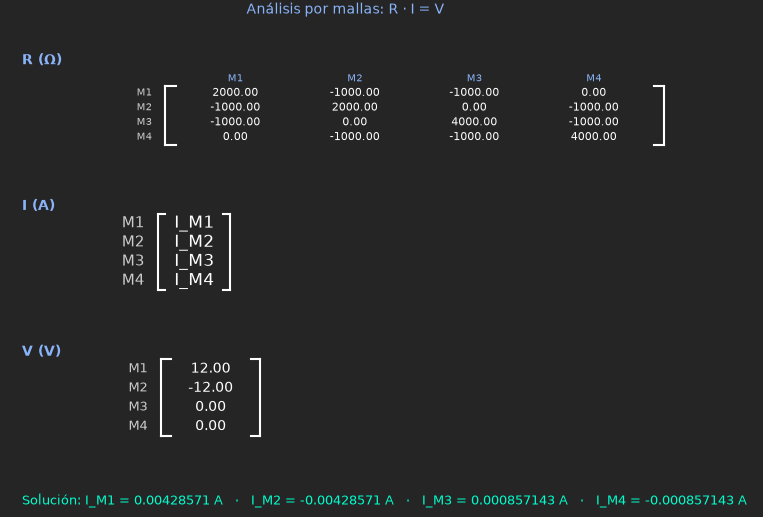
\includegraphics[width=0.78\textwidth]{../images/matrices_mallas.png}
  \caption{Panel de matrices del análisis por mallas. Se observan las matrices $R$, $I$ y $V$, la solución numérica y la rotulación $M_1, M_2, \ldots$ de las mallas.}
  \label{fig:matrices}
\end{figure*}

\begin{figure}[t]
  \centering
  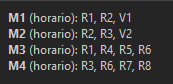
\includegraphics[width=0.92\columnwidth]{../images/leyenda_mallas.png}
  \caption{Leyenda de mallas detectadas. Cada malla indica su sentido de recorrido y los componentes que pertenecen a ella.}
  \label{fig:leyenda}
\end{figure}

% ------------------------------------------------------------------
% 5. Evidencia y resultados
% ------------------------------------------------------------------
\section{Evidencia y resultados}
\label{sec:evidencia}

La aplicación se probó con circuitos de una y dos mallas, con resistencias en serie, en paralelo y con ramas que no pertenecen a ninguna ventana. En el ejemplo de dos mallas usado durante la exposición, la herramienta reproduce los valores calculados a mano: $I_1 \approx 5.45$ mA e $I_2 \approx 2.18$ mA. La Figura~\ref{fig:lienzo} muestra el lienzo con un circuito dibujado y la Figura~\ref{fig:resultados} la tabla de resultados por componente.

\begin{figure}[t]
  \centering
  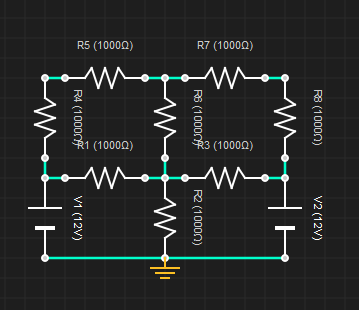
\includegraphics[width=0.90\columnwidth]{../images/lienzo.png}
  \caption{Lienzo con un circuito resistivo dibujado sobre la grilla. Los terminales que comparten celda forman un mismo nodo.}
  \label{fig:lienzo}
\end{figure}

\begin{figure}[t]
  \centering
  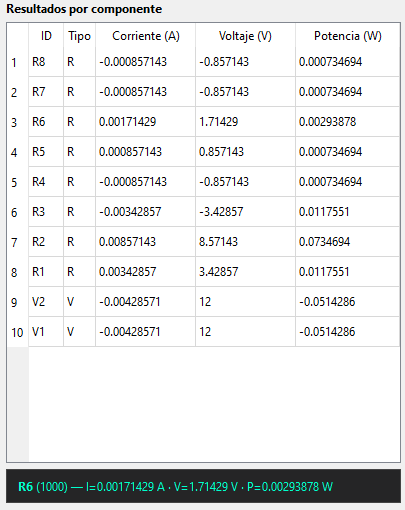
\includegraphics[width=0.78\columnwidth]{../images/resultados.png}
  \caption{Tabla de resultados. Para cada componente se muestran la corriente, la tensión y la potencia.}
  \label{fig:resultados}
\end{figure}

La validación del proyecto combina pruebas automatizadas y revisión de calidad. La Tabla~\ref{tab:evidencia} resume los resultados. Las 79 pruebas cubren el núcleo matemático, la detección de nodos, el comportamiento de imán, las conexiones por cable, los límites de componentes, el formato de las matrices y la integración con el lienzo. La revisión con Ruff no reportó hallazgos y la auditoría de dependencias no encontró vulnerabilidades conocidas. El ejecutable de Windows también se probó localmente, incluyendo el arranque desde la carpeta de distribución.

\begin{table}[t]
  \caption{Evidencia de verificación del proyecto.}
  \label{tab:evidencia}
  \centering
  \small
  \begin{tabular}{@{}ll@{}}
    \hline
    Aspecto & Resultado \\
    \hline
    Pruebas automatizadas & 79 aprobadas \\
    Estilo y errores estáticos & Ruff sin hallazgos \\
    Dependencias & Sin vulnerabilidades conocidas \\
    Empaquetado & Build de Windows probado \\
    \hline
  \end{tabular}
\end{table}

Además de la validación técnica, el proyecto se preparó como evidencia de una exposición de aproximadamente diez minutos y medio, repartida entre cinco integrantes. El guion de la exposición sigue el mismo hilo del informe: el circuito como sistema de ecuaciones, la construcción de $R \cdot I = V$, la geometría de las mallas, el ensamblado de la matriz y una demostración final. Las capturas de este documento sirven como respaldo si la demostración en vivo falla. El material completo del guion se encuentra en \texttt{docs/Guion\_Exposicion.md}, y el manual de uso en \texttt{Manual\_Usuario.md}.

% ------------------------------------------------------------------
% 6. Limitaciones y trabajo futuro
% ------------------------------------------------------------------
\section{Limitaciones y trabajo futuro}
\label{sec:limitaciones}

La versión actual tiene un alcance deliberadamente acotado. Trabaja solo con circuitos resistivos de corriente directa, con resistencias y fuentes de voltaje. No incluye corriente alterna, capacitores, inductores ni fuentes controladas. Además, impone un máximo de 20 resistencias y 3 fuentes por circuito, y muestra un aviso cuando se intenta superar ese límite. Estas restricciones mantienen la herramienta enfocada en los conceptos que se quieren enseñar y evitan que la interfaz se vuelva difícil de manejar en un curso introductorio.

Este informe y la exposición se centran en el análisis por mallas, que es el método construido a partir de la geometría del dibujo. La aplicación conserva otras opciones de análisis como apoyo interno, pero el material presentado se concentra en el recorrido que va del dibujo a la matriz $R \cdot I = V$.

Como trabajo futuro se plantean varias líneas. La primera es ampliar la compatibilidad con macOS y Linux, ya que el paquete probado está pensado para Windows. La segunda es automatizar la compilación y las pruebas con GitHub Actions, para que cada cambio genere un paquete verificable. La tercera es firmar digitalmente el ejecutable y reducir las advertencias de SmartScreen. También sería útil exportar los resultados a PDF o CSV, incorporar más tipos de componentes y permitir guardar y cargar circuitos desde un archivo.

% ------------------------------------------------------------------
% 7. Conclusión
% ------------------------------------------------------------------
\section{Conclusión}
\label{sec:conclusion}

Calc\_Resis\_AGBL demuestra que un circuito resistivo puede verse como un sistema lineal y que esa idea se puede hacer visible en una interfaz. El usuario dibuja, conecta y resuelve; la aplicación detecta la geometría, construye la matriz, obtiene la solución y presenta los resultados por componente. El valor educativo no está solamente en la respuesta numérica, sino en mostrar el recorrido completo: del dibujo a los nodos, de los nodos a las mallas, de las mallas a la matriz y de la matriz a la solución.

El proyecto cumple los objetivos propuestos para el curso: es una herramienta funcional, está documentado, incluye pruebas automatizadas y puede ejecutarse tanto desde el código fuente como desde un paquete de Windows. El repositorio de GitHub queda disponible para que otros estudiantes lo usen, lo revisen y lo amplíen.

% ------------------------------------------------------------------
% Agradecimientos
% ------------------------------------------------------------------
\section*{Agradecimientos}

Agradecemos a UCompensar y al grupo Juiciosos por el espacio y el acompañamiento para desarrollar este proyecto. También agradecemos a OpenCode y a los distintos modelos de inteligencia artificial que apoyaron la redacción, la revisión y la depuración del trabajo. Su uso fue supervisado por el equipo, que validó el código y los resultados con pruebas automatizadas y con la comparación de los ejemplos resueltos a mano.

% ------------------------------------------------------------------
% Referencias
% ------------------------------------------------------------------
\begin{thebibliography}{1}

\bibitem{kirchhoff1847}
G. Kirchhoff, ``Ueber die Aufl\"osung der Gleichungen, welche sich bei der Untersuchung der linearen Vertheilung galvanischer Str\"ome aufstellen lassen,'' \emph{Annalen der Physik und Chemie}, vol. 72, pp. 497--508, 1847.

\bibitem{nilsson2015}
J. W. Nilsson and S. A. Riedel, \emph{Electric Circuits}, 10th ed. Upper Saddle River, NJ, USA: Pearson, 2015.

\end{thebibliography}

\end{document}
